\documentclass[xcolor=dvipsnames]{beamer} 

\usepackage[latin1]{inputenc}
\usefonttheme[onlymath]{serif}
\usepackage{amsmath}
\usepackage{amsfonts}
\usepackage{amssymb}
\usepackage{amsthm}
\usepackage{latexsym,float}
\usepackage{times}
\usepackage[T1]{fontenc}
\usepackage{lmodern}

\usepackage{amscd}
\usepackage{amsfonts}

\setbeamertemplate{footline}[page number]{}
\setbeamertemplate{navigation symbols}{}
\newtheorem{proposition}[theorem]{Proposition}

\usepackage{algorithm,algorithmic}
\definecolorset{rgb}{}{}{darkred,0.8,0,0;darkgreen,0,0.5,0;darkblue,0,0,0.5}

\title{Asymptotically Exact, Embarrassingly Parallel MCMC}
\author{Willie Neiswanger, Chong Wang, Eric P. Xing}
\date{MCMC Journal Club \\ May 23 2018}

\begin{document}

\setlength{\unitlength}{\textwidth}  % measure in textwidths

\frame{\titlepage}

\frame{
\frametitle{Parallel MCMC}
\begin{itemize}
	\item Parallel chains: independent chains on full-data (slow burnin)% burnin
	\item Parallelize single chains: compute on a subset of data and exchange information at each iteration (communication overhead)% communication cost
\end{itemize}
}


\frame{
\frametitle{Proposed algorithm}
\begin{itemize}
\item Each machine has access to a portion of data
\item Each machine runs independent chains without communication (embarrassingly parallel)
\item Each machine can use any type of MCMC to generate samples
\item Combine samples to yield asymptotically exact full-data posterior samples
\end{itemize}
}

\frame{
\frametitle{Embarrassingly parallel MCMC}
\begin{itemize}
	\item Partition i.i.d data points $x^N$ into $M$ subsets $\{x^{n_1}, \dots, x^{n_M}\}$ % can be equal or not equal
	\item For machine $m = 1, \dots, M$, sample from \textit{subposterior} $p_m(\theta)$
	 $$p_m(\theta) \propto p(\theta)^{\frac{1}{M}} p(x^{n_m}\mid \theta)$$ % no communication, can be done using the same way as sampling from full data posterior
	\item Combine samples to form samples from an estimate of \textit{subposterior density product} $p_1 \dots p_M$ where
	 $$p_1 \dots p_M(\theta) \propto p(\theta \mid x^N)$$
\end{itemize}
}

\frame{
\frametitle{Combine subposterior samples}
\begin{itemize}
	\item Goal: get an estimate of subposterior density product $p_1\dots p_M(\theta)$, which is proportion to the full-data posterior
	\item Presented three estimators: parametric, nonparametric, and semiparametric
\end{itemize}
}

\frame{
\frametitle{Parametric estimator}
\begin{itemize}
\item Bayesian CLT: $p(\theta \mid x^N) \approx \mathcal{N}_d(\theta_0, F_N^{-1})$ as $N \to \infty$
\item Estimate each subposterior density with 
$$\widehat{p_m} = \mathcal{N}_d(\theta \mid \widehat{\mu}_m, \widehat{\Sigma}_m)$$
\item $\widehat{p_1\dots p_M}(\theta) = \widehat{p}_1 \dots \widehat{p}_M(\theta) \propto \mathcal{N}_d (\theta \mid \widehat{\mu}_M, \widehat{\Sigma}_M)$ %where $\widehat{\Sigma}_M = (\sum\limits_{m=1}^M \widehat{\Sigma}_m^{-1})^{-1}$ and
%$\widehat{\mu}_M = \widehat{\Sigma}_M (\sum\limits_{m=1}^{M} \widehat{\Sigma}_m^{-1} \widehat{\mu}_m)$
\item fast but asymptotically biased when posterior is non-Gaussian
\end{itemize}
}

\frame{
\frametitle{Nonparametric estimator}
\begin{itemize}
\item Given $T$ samples $\{\theta_{t_m}^m\}_{t_m=1}^T$, Gaussian KDE of subposterior
	$$\widehat{p}_m(\theta) = \frac{1}{T} \sum\limits_{t_m = 1}^T \mathcal{N}_d(\theta \mid \theta_{t_m}^m, h^2 I_d) $$
\item \begin{small}$\widehat{p_1\dots p_M}(\theta) = \widehat{p}_1 \dots \widehat{p}_M(\theta) %= \frac{1}{T^M} \prod\limits_{m=1}^M \sum\limits_{t_m=1}^T  \mathcal{N}_d(\theta \mid \theta_{t_m}^m, h^2 I_d)$
\propto \sum\limits_{t_1=1}^T \dots \sum\limits_{t_M=1}^T w_{t \cdot}\ \mathcal{N}_d(\theta \mid \bar{\theta}_{t \cdot}, \frac{h^2}{M} I_d) $\end{small}
\item Generate samples using IMG sampler from the mixture
\item Asymptotically exact, but slow to converge when $d$ is large
\end{itemize}
}

\frame{
\frametitle{Semiparametric estimator}
\begin{itemize}
	\item product of a parametric estimator $\widehat{f}_m(\theta)$ with a nonparametric estimator $\widehat{r}(\theta)$ of correction function $r(\theta) = \frac{p_m(\theta)}{\widehat{f}_m(\theta)}$
	
	$$\widehat{p}_m(\theta) = \widehat{f}_m(\theta) \widehat{r}(\theta) = \frac{1}{T} \sum\limits_{t_m=1}^T \frac{\mathcal{N}_d(\theta\mid \theta_{t_m}^m, h^2 I_d) \mathcal{N}_d(\theta \mid \widehat{\mu}_m, \widehat{\Sigma}_m)}{\mathcal{N}_d (\theta_{t_m}^m \mid \widehat{\mu}_m, \widehat{\Sigma}_m)}$$
	
	\item  \begin{small}$\widehat{p_1\dots p_M}(\theta) = \widehat{p}_1 \dots \widehat{p}_M(\theta) \propto \sum\limits_{t_1 = 1}^T \dots \sum\limits_{t_M=1}^T W_{t\cdot} \mathcal{N}_d(\theta \mid \mu_{t\cdot}, \Sigma_{t\cdot}) $\end{small}
	\item Generate samples using IMG similarly as in nonparametric
\end{itemize}
}

\frame{
\frametitle{Method complexity and density product estimate convergence}
\begin{itemize}
	\item parallel MCMC chains: $O(dTM)$ + combination phase: $O(dTM)$
	\item MCMC phase and combination phase can also be performed in parallel
	\item Showed mean square consistency of nonparametric and semiparametric estimator:
	
		$$\sup\limits_{p_1, \dots, p_M \in \mathcal{P}(\beta, L)} \mathbb{E}[\int (\widehat{p_1\dots p_M}(\theta) - p_1 \dots p_M(\theta))^2 d\theta] \leq \frac{c}{T^{2\beta /(2\beta + d)}}$$ for some $c > 0$ and $0 < h \leq 1$
\end{itemize}
}

\frame{
\frametitle{Method scope}
\begin{itemize}
	\item Posterior distributions over finite-dimensional real spaces
	\item Not yet extended to infinite dimensional models (nonparametric Bayesian models), distribution over the simplex (LDA)
\end{itemize}
}

\frame{
\frametitle{Empirical study}
\framesubtitle{logistic regression: simulated data}
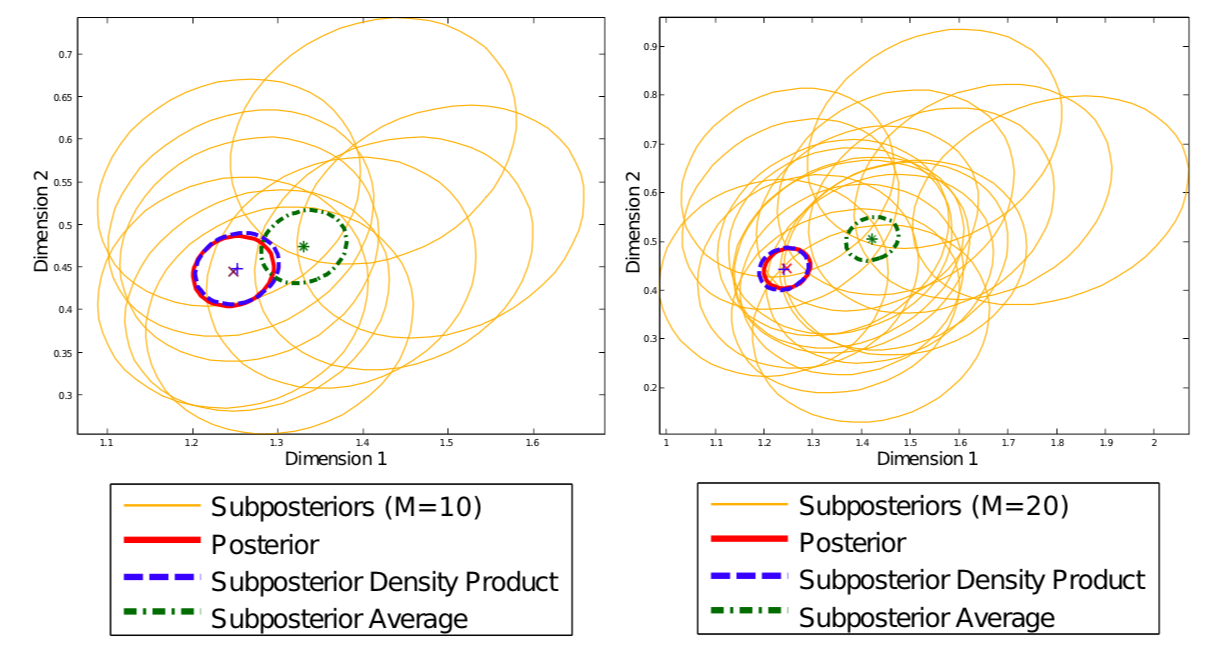
\includegraphics[width=0.5\textwidth]{figures/subposterior}
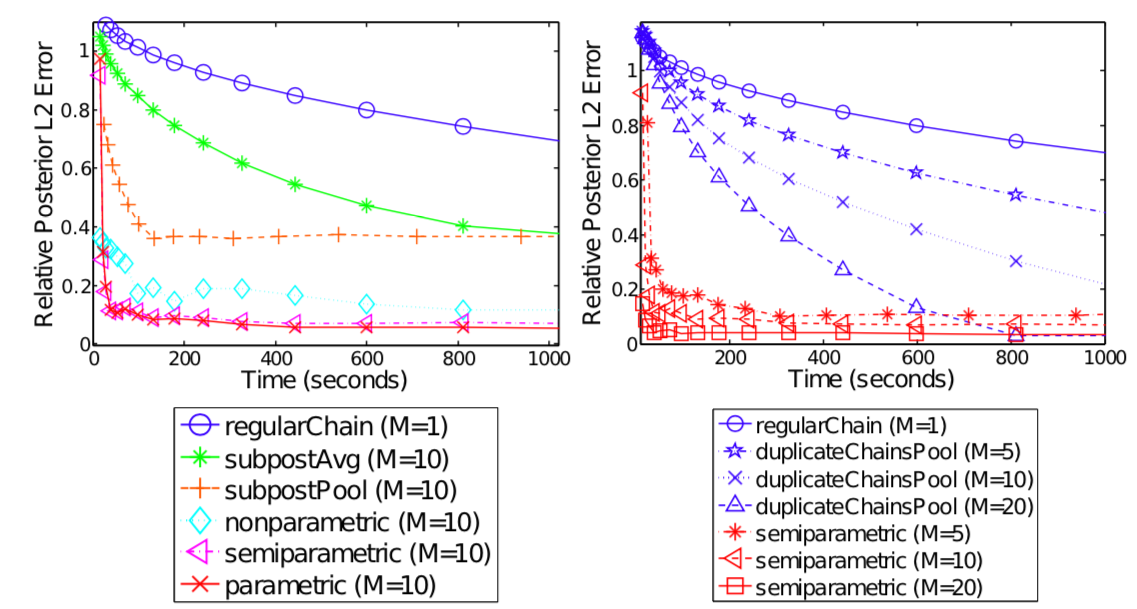
\includegraphics[width=0.5\textwidth]{figures/L2error}

\begin{small}
\begin{align}
N &= 5 \times 10^4, \quad d = 50, \quad M = 10 \nonumber\\
X_{ij} &\sim \mathcal{N}(0, 1), \quad \beta_j \sim \mathcal{N}(0, 1) \nonumber\\
Y_i &\sim \text{Bernoulli}(\text{logit}^{-1}(X_i\boldsymbol{\beta})) \nonumber \\
d_2(p, \hat{p}) &= || p - \hat{p} ||^2 = (\int (p(\theta) - \hat{p}(\theta))^2 d\theta)^{1/2} \nonumber
\end{align}
\end{small}
}

\frame{
\frametitle{Empirical study}
\framesubtitle{logistic regression: real world data \textit{covtype}}
\begin{columns}
\begin{column}{0.5\textwidth}
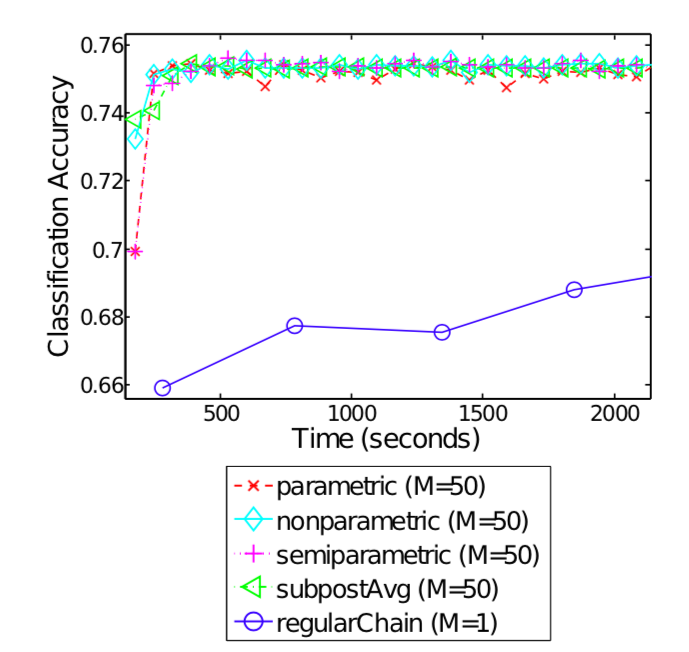
\includegraphics[width=0.9\textwidth]{figures/realdata}
\end{column}
\begin{column}{0.5\textwidth}
\begin{align}
	&N = 581012, \quad d = 54, \quad M = 50 \nonumber\\
	&P(y \mid x, y^N, x^N) \approx \frac{1}{S} \sum\limits_{s=1}^S P(y \mid x, \beta_s) \nonumber\\
	 &P(y \mid x, \beta_s) \sim \text{Bernoulli}(\text{logit}^{-1}(x^T\beta_s)) \nonumber
\end{align}
\end{column}
\end{columns}
}

\frame{
\frametitle{Empirical study}
\framesubtitle{Scalability with dimension}
\begin{center}
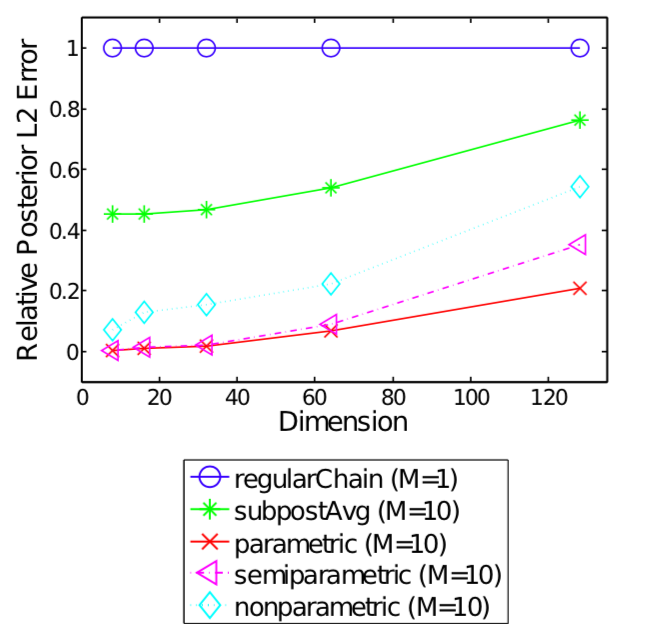
\includegraphics[width=0.6\textwidth]{figures/scalability}
\end{center}
}

\frame{
\frametitle{Empirical study}
\framesubtitle{Guassian mixture models}
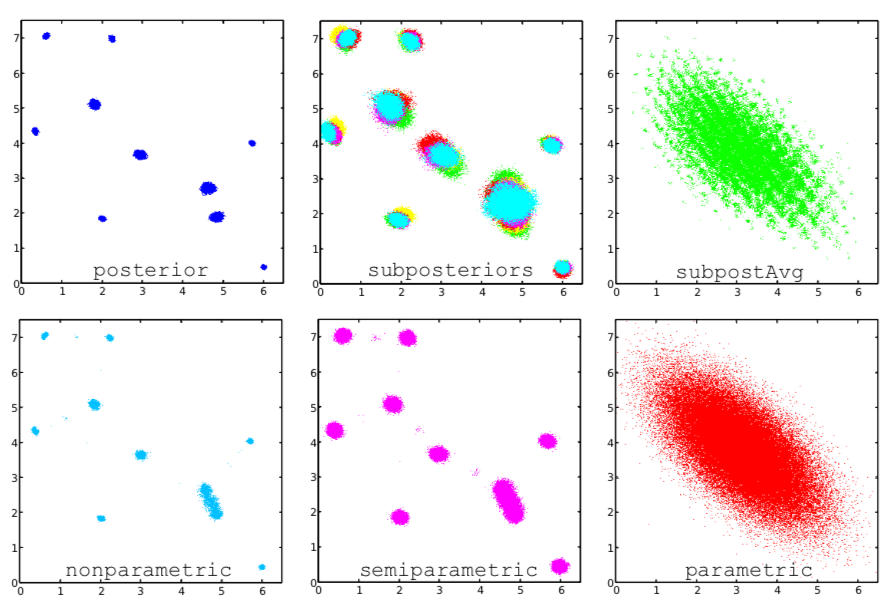
\includegraphics[width=0.6\textwidth]{figures/mixtureposterior}
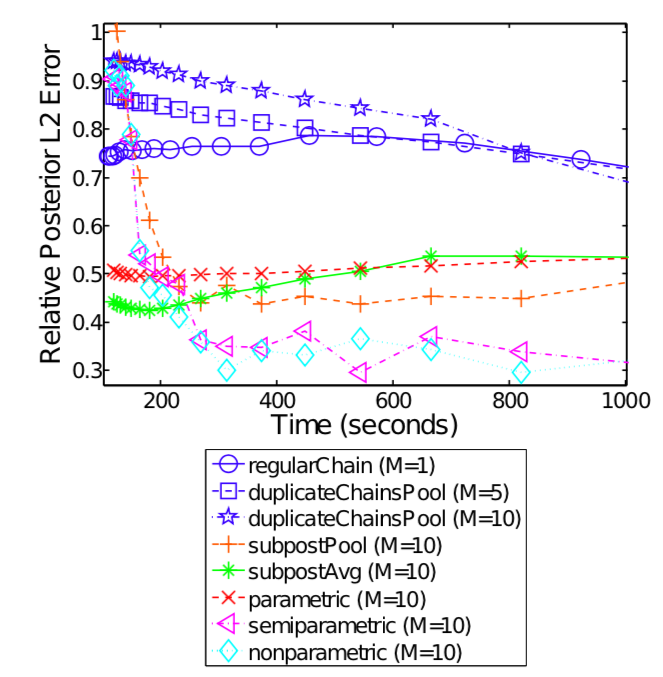
\includegraphics[width=0.4\textwidth]{figures/mixtureaccuracy}
\begin{align}
	\text{10\ 2-d\ Guassians}, \quad N = 5 \times 10^4, \quad M = 10 \nonumber
\end{align}
}

\frame{
\frametitle{Empirical study}
\framesubtitle{HIerarchical Poisson-gamma models}
\begin{columns}
\begin{column}{0.5\textwidth}
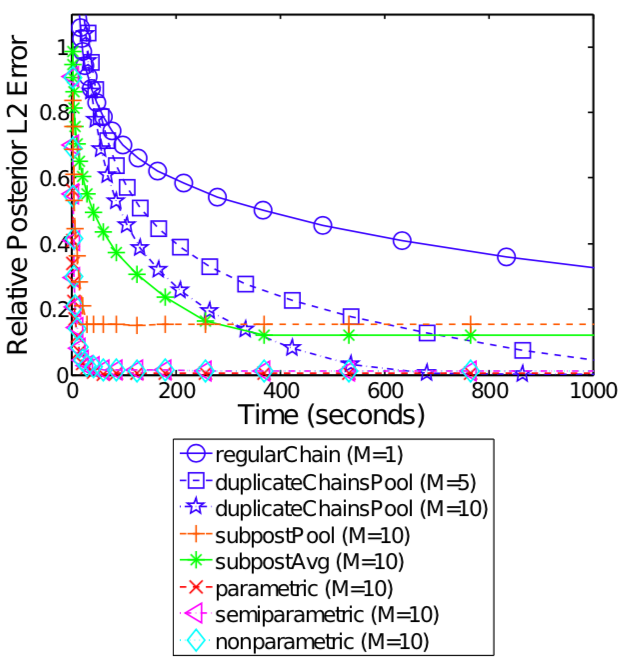
\includegraphics[width=\textwidth]{figures/hierarchicalaccuracy}
\end{column}
\begin{column}{0.5\textwidth}
\begin{align}
N &= 5 \times 10^4, \quad M = 10 \nonumber\\
a &\sim \text{Exponential}(\lambda) \nonumber\\
b &\sim \text{Gamma}(\alpha, \beta) \nonumber\\
q_i &\sim\text{Gamma}(a, b) \nonumber\\
x_i &\sim \text{Poisson}(q_it_i), \quad i = 1, \dots, N \nonumber
\end{align}
\end{column}
\end{columns}
}

\frame{
\frametitle{Summary}
\begin{itemize}
	\item faster burnin by only operating on a subset of data (cf. parallel chains)
	\item faster sampling since no communication is involved (cf. parallelized single chain)
	\item ideal for MapReduce settings
	\item only works when posterior samples are real and unconstrained 
\end{itemize}
}

\frame{
\frametitle{IMG procedure}
\centering
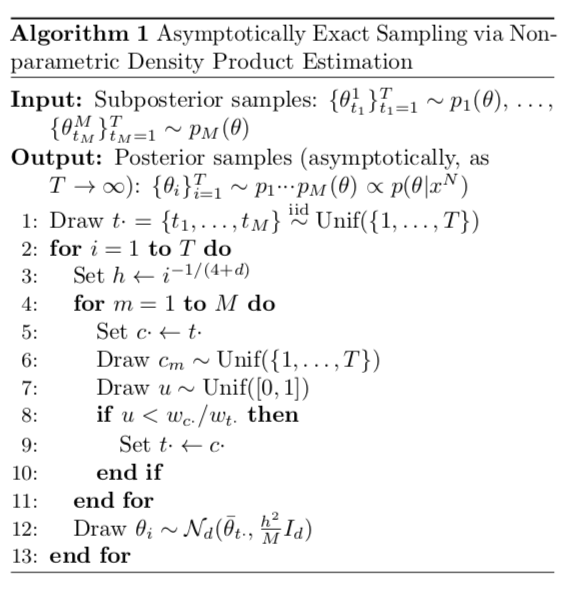
\includegraphics[width=0.6\textwidth]{figures/IMG}
}

\end{document}
